\documentclass{article}
\usepackage[utf8]{inputenc}
\usepackage[greek,english]{babel}
\usepackage{alphabeta}
\usepackage{fancyhdr}
\usepackage{listings}
\usepackage{mathtools}
\usepackage{xcolor}
\usepackage{biblatex}
\usepackage[left=2cm,right=2cm]{geometry}

\lstset {
        basicstyle=\ttfamily,
        columns=fullflexible,
        breaklines=true,
        keepspaces=true
}

\title{Σχεδίαση Ψηφιακών Συστημάτων - Εργασία Θεωρίας (Μέρος 7)}
\author{Χρήστος Μαργιώλης}
\date{Ιούλιος 2020}

\begin{document}

\begin{titlepage}
        \maketitle
\end{titlepage}

\renewcommand{\contentsname}{Περιεχόμενα}
\tableofcontents

\section{Κώδικας και τεκμηρίωση}

Για καλύτερη κατανόηση του κώδικα του MIPS, παραθέτω και τις υλοποιήσεις (ξανά)
όλων των κυκλωμάτων που χρησιμοποιήθηκαν. Μερικά από τα κυκλώματα υπέστησαν μικρές 
τροποιήσεις.

\subsection{\lstinline{alu.vhd}}

Αριθμητική και λογική μονάδα. \\

\lstinputlisting[language=VHDL]{../alu.vhd}
\pagebreak

\subsection{\lstinline{regfile_ext.vhd}}

Register file. \\

\lstinputlisting[language=VHDL]{../regfile_ext.vhd}
\pagebreak

\subsection{\lstinline{instrmem.vhd}}

Μνήμη εντολών. \\

\lstinputlisting[language=VHDL]{../instrmem.vhd}
\pagebreak

\subsection{\lstinline{ctrl.vhd}}

Μονάδα ελέγχου. \\

\lstinputlisting[language=VHDL]{../ctrl.vhd}
\pagebreak

\subsection{\lstinline{alu_ctrl.vhd}}

Μονάδα ελέγχου ALU. \\

\lstinputlisting[language=VHDL]{../alu_ctrl.vhd}
\pagebreak

\subsection{\lstinline{adder32.vhd}}

Αθροιστής 32-bit. \\

\lstinputlisting[language=VHDL]{../adder32.vhd}
\pagebreak

\subsection{\lstinline{pc.vhd}}

Program counter. \\

\lstinputlisting[language=VHDL]{../pc.vhd}
\pagebreak

\subsection{\lstinline{mips.vhd}}

'Οπως λέει η εκφώνηση, ο MIPS έχει μόνο δύο εισόδους: τον ορολογιακό παλμό και
το σήμα reset, και δεν έχει εξόδους. Στην αρχιτεκτονική του δηλώνουμε ως components
όλα τα παραπάνω κυκλώματα. 'Επειτα δημιουργούμε βοηθητικά σήματα για το πέρασμα
αποτελεσμάτων από το ένα κύκλωμα στο άλλο. \\

\lstinputlisting[language=VHDL]{../mips.vhd}
\pagebreak

\subsection{\lstinline{mips_tb.vhd}}

Testbench για δοκιμή του MIPS. \\

\lstinputlisting[language=VHDL]{../mips_tb.vhd}
\pagebreak

\section{Εκτέλεση}

\subsection{\lstinline{mips_tb}}

Στην εκφώνηση της άσκησης ζητήθηκε ο MIPS να έχει μόνο τον ορολογιακό παλμό
και το reset ως εισόδους, και όχι εξόδο. Παρ'όλα αυτά για την καλύτερη κατανόηση
του κυκλώματος, έβαλα επιπλέον σήματα στο κύκλωμα (δεν περιλαμβάνονται στον
κώδικα πια εφόσον δεν ζητούνται). \\

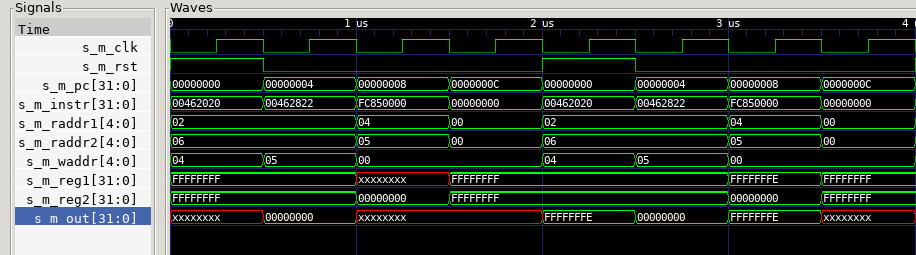
\includegraphics[width=\textwidth]{res/mips.png}

\end{document}
